\chapter{Bluetooth}
\label{chap:bluetooth}

Bluetooth is an IEEE standard(802.15.1+) registerd in 1999 and designed as a "wireless cable" more 
than a general-purpose wireless network. In fact, it is intended to be short-range, low-power, 
ubiquitous, and inexpensive, being roughly a wireless USB in capability and ubiquity.\\
Nowadays, the standard has quite evolved and it is possible to have a Bluetooth network.\\
\begin{figure}[H]
  \centering
  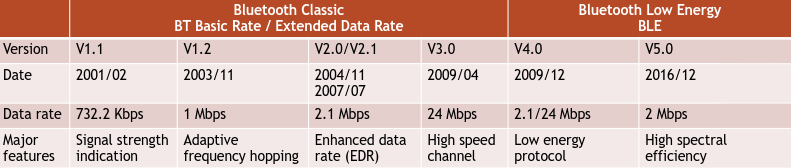
\includegraphics[width=0.7\textwidth]{img/wireless/bluetooth versions.png}
  \caption{Bluetooth versions}
\end{figure}
\begin{section}{Bluetooth networks}
  There are actually different types of Bluetooth networks.
  \begin{subsection}{Piconet}
    A piconet is a network of devices(ad-hoc) connected using Bluetooth technology withing a small area. 
    One device acts as the master and the other devices act as slaves. Up to seven slaves can be 
    connected to one master. The master controls the channel access of the slaves.\\
    The communication is strictly between a master and a slave at a time, no slave-to-slave communication
    is allowed.\\
    \begin{figure}[H]
      \centering
      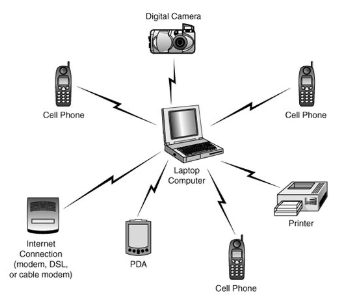
\includegraphics[width=0.4\textwidth]{img/wireless/piconet.png}
      \caption{A piconet bluetooth network}
    \end{figure}
  \end{subsection}

  \begin{subsection}{Scatternet}
    A scatternet is a network of piconets. A device in one piconet can be a slave in another piconet. 
    This allows the devices to communicate with each other even if they are not in the same piconet.\\
    One node can't be a master in two piconets at the same time and it may be a slave in one piconet and
    a master in another.\\
    \begin{figure}[H]
      \centering
      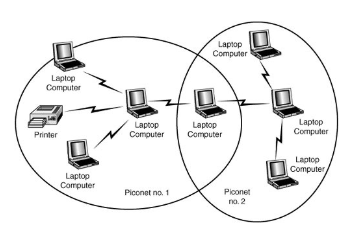
\includegraphics[width=0.4\textwidth]{img/wireless/scatternet.png}
      \caption{A scatternet bluetooth network}
    \end{figure}
  \end{subsection}

  \begin{subsection}{Personal Area Network}
    A Personal Area Network(PAN) is a network of devices within a range of 10 meters, using the bluetooth
    technology, in this case. It is meant to replace the cables between devices, like a wireless USB.\\
    It works in the 2.4-5 GHz frequency band and it is a low-power network, being able to transmit
    up to 3Mbps.\\
    This kind of netawork is an ad-hoc one, with a master controller and many clients, meaning that 
    it requires a polling mechanism to avoid collisions. It actually implements a TDM+FDM, with a 
    TDM slots of 625 ms and FDM over 79 channels in BT classic and 40 channels in BLE, while also 
    implmenting a frequency hopping mechanism.\\
    For energy saving, the devices can enter a low-power mode, where they can be woken up by the master
    controller. This network can also be \textit{self-assembling}, meaning that the devices can
    automatically connect to each other and set up a network.\\
    This requires means for authentication, authorization, confidentiality, and integrity.\\
  \end{subsection}
\end{section}

\begin{section}{Protocol stack}
  The protocol stack for the different versions of Bluetooth is shown in figure \ref{fig:bluetooth stack}.
  \begin{figure}[H]
    \centering
    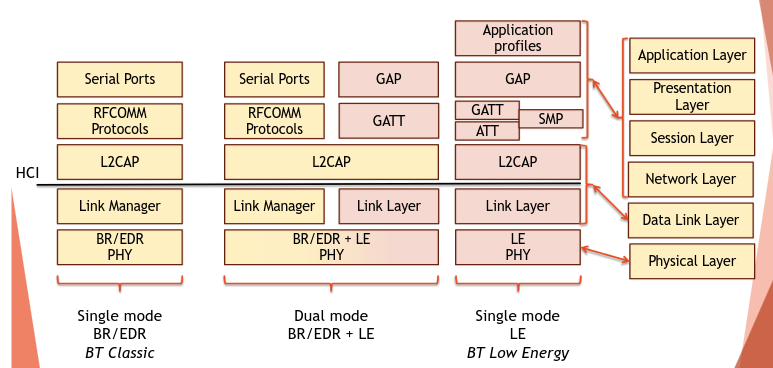
\includegraphics[width=0.7\textwidth]{img/wireless/bluetooth protocol tack.png}
    \caption{Bluetooth protocol stack}
    \label{fig:bluetooth stack}
  \end{figure}
  We will mainly focus on the more recent versions of Bluetooth(Low Energy).
  In bluetooth LE, there are 3 main specifications:
  \begin{itemize}
    \item the core specifications, which defines the architecture of the technology, the key features
      and the formal procedures, as well ad the protocols. 
    \item the profiles, which define the role of the device(client/server), its behavior and the
      transmitted data.
    \item the services, which define service group characteristics and descriptors, providing a 
      formal description of the data exchanged between devices.
    \begin{figure}[H]
      \centering
      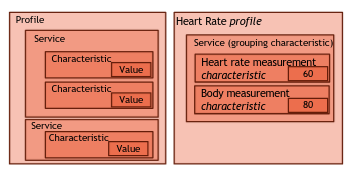
\includegraphics[width=0.5\textwidth]{img/wireless/bluetooth services format.png}
      \caption{An example of the data structure of some services}
    \end{figure}
  \end{itemize}
  \begin{subsection}{The host stack}
    The host stack is the software stack that runs on the host device, which is the device that 
    controls the communication. 
    \begin{figure}[H]
      \centering
      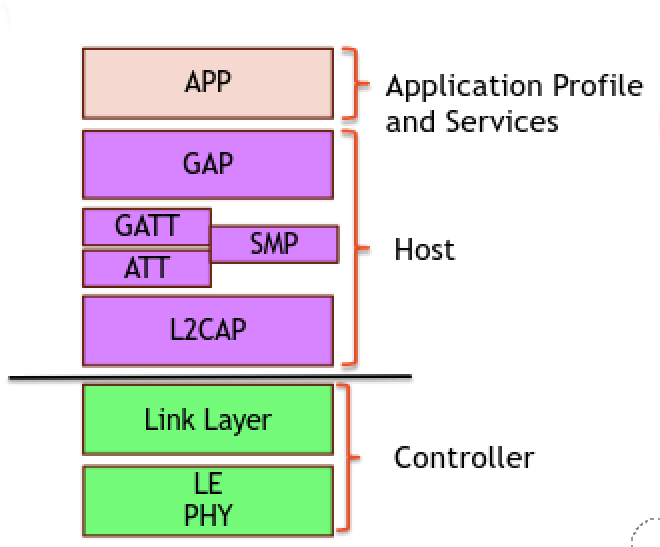
\includegraphics[width=0.4\textwidth]{img/wireless/bluetooth host stack.png}
      \caption{Bluetooth host stack}
    \end{figure}
    \begin{subsubsection}{Generic Access Profile}
      The Generic Access Profile(GAP) defines the roles, models, and procedures of a Bluetooth device.
      It provides communication channel between the devices, allowing them to:
      \begin{itemize}
        \item discover each other
        \item establish a link 
        \item terminate a link
        \item initialize the security features
        \item configure the device
      \end{itemize}
    \end{subsubsection}
    \begin{subsubsection}{Device states}
      The device can be in different states during the communication process:
      \begin{itemize}
      \item Standby: The device is in the initial idle state upon reset
      \item Advertiser: The device is advertising with specific data letting any initiating devices
        know that it is a connectible device. Messages contain the device address and some
        additional data, e.g. device name
      \item Scanner: When receiving the advertisement, the scanning device sends a scan request to
        the advertiser. The advertiser responds with a scan response. This process is called device
        discovery
      \item Initiator: When initiating, the initiator must specify a peer device address to which to
        connect. Suppose an advertisement is received matching the address of the peer device. In
        that case, the initiating device requests to establish a connection (link) with the
        advertising device specifying the Connection Parameters
      \item Slave/Master: Connection is formed. The device functions as a slave if the advertiser
        and a master if the initiator
      \end{itemize}
      \begin{figure}[H]
        \centering
        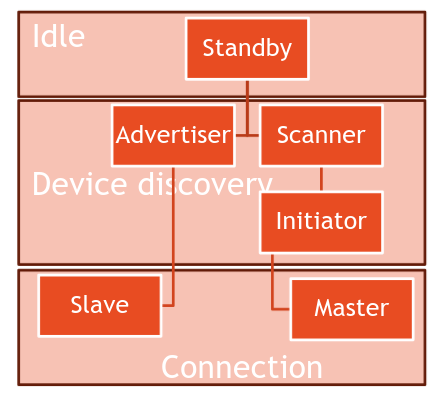
\includegraphics[width=0.4\textwidth]{img/wireless/bluethooth device states.png}
        \caption{Bluetooth device states}
      \end{figure}

    \end{subsubsection}
    \begin{subsubsection}{Generic attribute}
      The generic attribute(GATT) allows the devices to exchange data, providing data communication
      between two connected devices.\\ 
      Data is exchanged as a relationship data-attribute using a client-server model. The GATT-server
      accepts incoming commands and requests from a client and sends responses, indications, and notifications.
      The GATT-Client initiates commands and requests towards the server, receive responses, indications, and notifications.
    \end{subsubsection}

    \begin{subsubsection}{Attribute}
      The attribute level(ATT) transfers a single attribute data between the client and the server
      in the GATT-based profiles.\\
      Data can be accessed in different ways(read, wire, delete, \dots) and is organized in the form
      of attributes, each one having:
      \begin{itemize}
        \item an handle of 16-bits, which defines the type 
        \item an universally unique identifier(UUID)
        \item a value
        \item a set of permissions
      \end{itemize}
    \end{subsubsection}

    \begin{subsubsection}{L2CAP}
      L2CAP, or Logical Link Control and Adaptation Protocol, is the equivalent of the data link layer,
      which encapsulates data from the Bluetooth LE higher layers into the standard Bluetooth LE
      packet format for transmission according to the link configuration specified at the ATT and
      SMP layers.\\
      It provides means for:
      \begin{itemize}
        \item Protocol multiplexing
        \item Segmentation, and reassembly (SDU up to 64kB long)
        \item Retransmission
        \item Flow control
      \end{itemize}
      Under it, the HCI layer is responsible for the communication between the host and the
      controller, providing a command interface to the controller and a data interface to the host.

    \end{subsubsection}

  \end{subsection}
  \begin{subsection}{Service Discovery protocol}
    There's a middleware protocol that is not part of the Bluetooth stack, but it is used to discover
    the services provided by a device. This is the \textbf{Service Discovery Protocol}(SDP), which
    allows the devices to discover the services provided by another device, as well as their 
    associated parameters.\\
    It includes many phases, which are all optional.
    \begin{figure}[H]
      \centering
      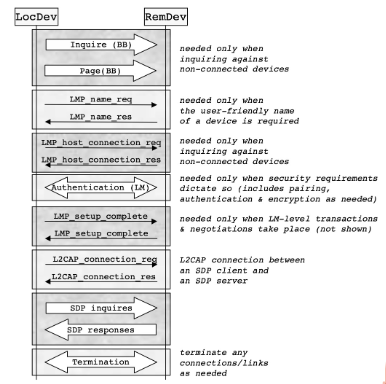
\includegraphics[width=0.5\textwidth]{img/wireless/bluetooth sdp.png}
      \caption{The messages exchanged during the SDP}
    \end{figure}
  \end{subsection}

  \begin{subsection}{The controller part}
    The controller part of the Bluetooth stack is the one that manages the physical layer and the
    link layer, allowing the host to communicate with the hardware.\\
    It is made up of 3 main components.
    \begin{subsubsection}{Host controller interface}
      The host controller interface(HCI) is the interface between the host and the controller, 
      providing a command interface to the controller and a data interface to the host.\\
      It defines a set of commands, events, and parameters that are used for the transmission and 
      the reception of data.\\
      When receiving packets from the controller, the HCI extracts raw data at the controller to
      send to the host.
    \end{subsubsection}
    \begin{subsubsection}{Link layer}
      The link layer is the one that manages the physical layer, providing the means for the 
      communication between the devices.\\
      It mainly manages the state of the link and defines the role of the device in the
      communication(Central, Pheripheral, Advertiser or Scanner).
    \end{subsubsection}
    \begin{subsubsection}{Physical layer}
      The physical layer is the one that manages the physical communication between the devices.
      It is responsible for the modulation, the frequency hopping, the power control, and the 
      encryption of the data.\\
      This layer quite differs between the different versions of Bluetooth( mainly BTL and BLE), but 
      the same principles are applied(Frequency hopping-Spread Spectrum).\\
      Both versions still use the same ISM(Industrial, Scientific, and Medical) band of 2.4 GHz to
      2.485 GHz, which is quite crowded, meaning that a lot of interference has to be managed.\\
      The first versions of Bluetooth(BR/EDR) use a frequency hopping mechanism with 79 channels of 
      1 MHz each, while more recent versions(BT 1.2+) uses adaptive frequency hopping(AHN) to avoid
      channels with interference, which is quite a bad idea in crowded scenarios.\\

      It implements forward error correction(FEC), which is a mechanism to correct errors in the
      data, using parity bits. FEC have 2 options: 
      \begin{itemize}
        \item 1/3 rate FEC, which means that each bit it sent 3 times, with 2 parity bits
        \item 2/3 rate FEC, which means that each sequence of 10 bits have 5 parity bits
          using a shortened Hamming code(10,15)
      \end{itemize}
      The standard also allows for the implementation of retransmission
      and automatic repeat request(ARQ) mechanisms, while also providing means for CRC and
      awcknowledgments.\\
      It also provides means for flushing the packets that are waiting an awcknowledgment, which
      can be useful in some cases, like audio streams.\\

      As for frequency modulation, the standard uses GFSK(Gaussian Frequency Shift Keying) for the
      data, forming a phase shift to encode the data.\\
      This schema provide a basic rate of 1Mbps, which can be increased doing differential quadrature
      phase shift keying(DQPSK) or Key Shift Keyring(PSK) to 3Mbps.\\

      Bluetooth is also able to use more frequency space than needed for the data rate, to spread the
      signal and make it more resilient to noise and interference. This is called spread spectrum
      and it is implemented using frequency hopping(could also have used CMDA).\\
      Frequency hopping is exactly what it sounds like: a channel is divided into smaller ones, and 
      for each time slot, the device changes the channel. 

      \begin{figure}[H]
        \centering
        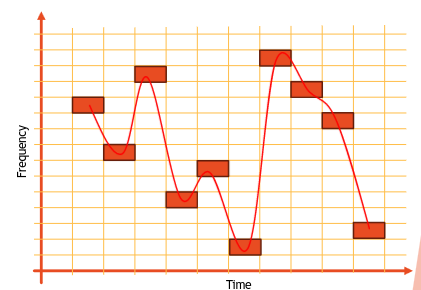
\includegraphics[width=0.5\textwidth]{img/wireless/frequency hopping.png}
        \caption{Bluetooth frequency hopping}
      \end{figure}
    This technique needs means for synchronization between the devices, which is done using a
    pre-detemined sequence of channels or announced by the master.\\

    A clock 312.5 $\mu$s long, dictated by the master, which is shared with the slaves.
    Two ticks can be grouped in a slot, which can be grouped, in a pair of 2, to form a slot pair,
    where the master send in the even slots and the slaves in the odd ones.\\
    Packets can be sent in 1, 3 or 5 slots.

    \begin{figure}[H]
      \centering
      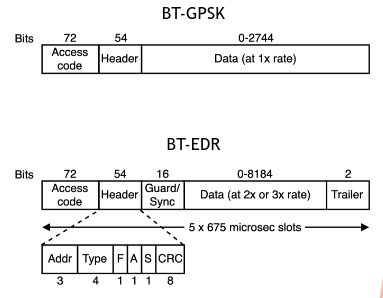
\includegraphics[width=0.5\textwidth]{img/wireless/bluetooth frame.png}
      \caption{The structure of a Bluetooth frame}
    \end{figure}
    \end{subsubsection}

  \end{subsection}
\end{section}

